\documentclass[%
 reprint,
%superscriptaddress,
%groupedaddress,
%unsortedaddress,
%runinaddress,
%frontmatterverbose, 
%preprint,
%showpacs,preprintnumbers,
%nofootinbib,
%nobibnotes,
%bibnotes,
 amsmath,amssymb,
 aps,
 pra,
%prb,
%rmp,
%prstab,
%prstper,
%floatfix,
]{revtex4-1}

\usepackage{graphicx}% Include figure files
\usepackage{dcolumn}% Align table columns on decimal point
%\usepackage{bm}% bold math
\usepackage{fullpage}
\usepackage{epsfig}
\usepackage{amsmath}
\usepackage{amsfonts}
\usepackage{amssymb}
\usepackage{float}
\usepackage{pstricks}
\usepackage{cancel}
\usepackage{lipsum}
%\usepackage[nottoc,numbib]{tocbibind} %Uncomment for bibliography to be its own numbered section
\usepackage{units}
\usepackage{listings}

\graphicspath{{../plots/}}

\begin{document}

\preprint{APS/123-QED}

\title{\textbf{Lab Report: Compton Scattering} \\ \small{An Investigation of the Angular Dependence of the Scattering Probability for Photons}}
\author{Joshua LaBounty}
\author{Thomas Krahulik}
\affiliation{Stony Brook University --- PHY 445}

\date{\today}

\begin{abstract}
	In this experiment, we test the classical Thompson Formula (Eq. \ref{eq:thompson}) against the Klein-Nishina Formula (Eq. \ref{eq:kn}), its quantum mechanical counterpart. At small angles, the two formulae agree quite well, but at large $\theta$ we see a significant deviation. In order to accomplish this, we look at Compton Scattering of $\gamma$-ray photons produced from the decay of a $^{137}$Cs source. We measure the angular dependence of the scattering probability $d\sigma / d\Omega$ in Aluminum at multiple angles ranging from $0^\circ - 110^\circ$ using a NaI(Tl) scintillating detector. We also use this phenomenon to measure the mass of the electron and compare the number of free electrons in two different media: Copper and Aluminum.
\end{abstract}
\maketitle

\section{Background and Review of Previous Work}

In the early 1920s, A. H. Compton, discovered something peculiar in his study of X-ray scattering. He found that the frequency (and thus the energy) of X-rays decreased after scattering off free electrons in a medium. This result is not consistent with the classical electromagnetic theory of light, as the magnitude of the electromagnetic field cannot be altered by the change in direction implicit in the scattering process. However, by considering the concept of light quanta (photons), Compton was able to build a model of the interaction between the incident photons and electrons using conservation of energy and momentum. In particular, he derived a form of the following relation:
\begin{gather}\label{eq:energy_scatter}
	E_\gamma ' = \frac{E_\gamma}{1 + \frac{E_\gamma}{m_e c^2} (1 - \cos{\theta})}
\end{gather}
This relates the incident energy of the photon with its final energy and the scattering angle. This relation, once shown experimentally to be true, was seen as major evidence in favor of the theory of light quanta. Through its derivation (see Appendix \ref{section:derivation}), it also provides a direct link between the wavelength and momentum of such quanta. Thus experiments which validate the formula also implicitly validate this crucial relation.

Another facet of Compton's work with X-rays is his examination of the scattering angle. He found that the theoretical scattering probability (which he expressed in terms of $I/I_0$ and we look at as $d\sigma / d\Omega$) was inconsistent with the Thompson prediction:
\begin{equation}\label{eq:thompson}
	\frac{d \sigma}{d \Omega}_{Th} = \frac{r_0^2}{2}(1+\cos^2{\theta})
\end{equation}
Instead he found that, once again, classical theory was inadequate for describing these quantum phenomena. At low angles, it agrees relatively well, but it fails as the angle of the detector relative to the source increases. It wasn't until 1928 that Klein and Nishina, using quantum electrodynamics, derived a formula which included not only quantum effects but also relativistic corrections\cite{kn_paper_original, eisberg}:
\begin{gather}
	\frac{d \sigma}{d \Omega}_{KN} = \frac{r_0^2}{2} \frac{1 + \cos^2{\theta}}{[1 + \gamma(1 - \cos{\theta})]^2} \nonumber * ~~~~~~~~~~~~ \\
	\left[ 1 + \frac{\gamma^2(1 - \cos{\theta})^2}{(1 + \cos^2{\theta})(1+ \gamma(1 - \cos{\theta}))}\right] 
	\label{eq:kn}
\end{gather}
where $\gamma = h\nu / m_e c^2$. Looking at these formulae, we can see that when $\gamma \ll 1$ Klein-Nishina will converge to the classical Thompson formula. This approximation holds for extremely low energy photons, from radio up to the visible spectrum, but fails as one reaches x-rays and $\gamma$-rays. A comparison of the angular dependence of these two equations for out setup can be seen in Figure \ref{KN_vs_Thompson_Theory}.

This particular experiment, and its results, are well documented in literature. Milissinos\cite{milissinos} describes a procedure for determining $d\sigma / d\Omega$ which is nearly identical to ours, and which was performed in 1962. This same investigation of $d\sigma / d\Omega$ has since been verified many times over \cite{angle_1, angle_2, angle_3}. The implications for physics are profound. It proves that light is primarily a quantum phenomenon, and cannot be completely explained by classical mechanics, as Thompson Scattering attempts to do. Compton scattering is still a valuable tool in order to explain a number of important phenomenon. In particular, the dominant source of opacity in a number of astrophysical phenomena (Black Holes, Neutron Stars, Nebulae, etc.) is Compton Scattering \cite{nstars}. Thus, in order to build models of these important foci of modern astronomical research, Compton scattering must be understood in depth. New research is also currently being undertaken to make further quantum mechanical corrections to our understanding of Compton scattering \cite{comptonresearch}.

The technique for measuring the electron mass is also well documented, and has been repeated with some alterations by students all over the world \cite{emass_1, emass_2, emass_3}. But the basic underlying truth of the experiment is unchanged: we can use a form of Equation \ref{eq:energy_scatter} to relate the electron mass with the scattering angle $\theta$ and the energy of the scattered $\gamma$-ray $E_\gamma '$. This method provided one of the earliest accurate measurements of the electron mass. We will also use this technique to compare the number of free electrons in two different materials, and compare the results with our assumption that all the electrons in the metal are free. The number of free electrons in a material is an important quantity to know in the world of both electronics and chemistry, because it not only effects how conductive a metal is but also how it will behave in any number of chemical reactions.

Below we detail the setup used to measure all of these quantities.

\section{Experimental Setup}

The source of the $\gamma$-rays for this experiment is a $^{137}$Cs sample, measured to emit $300~\mu Ci$ of radiation in 1978 and now emitting only $116~\mu Ci$ due to its decay, completely encased in lead save for a small aperture. This aperture is in line with the $0^\circ$ line on our table. On the other end of this experiment we have a movable detector. This detector consists of a NaI(Tl) scintillating crystal permanently bonded to a photomultiplier and a pre-amplifier. This detector is mounted on a movable platform which pivots around a point on the $0^\circ$ axis. Marks on the table allow us to rotate the detector semi-precisely about this axis to arbitrary angles. Also on this pivot is a mounting point for our scatterers, which consist of Aluminum and Copper cylinders with a hole drilled directly in the center. 

With the scatterer in place, the $\gamma$-rays which are emitted by the $^{137}$Cs pass through the aperture, scatter off electrons in the Al or Cu cylinders, and then pass into the NaI(Tl) crystal. These $\gamma$-rays produce scintillation photons proportional to their energy in the NaI(Tl) scintillation crystal. These scintillation photons are picked up as an electric signal by the photomultiplier, and then through two levels of amplification before being output to the Multi-Channel Analyzer (MCA). The MCA reconstructs the energy of the incident $\gamma$-rays from the signals and plots a histogram of Numbers of Photons detected vs. Bin Number (where the Bin Number corresponds to an photon energy). From there, the information is saved in a format which can be read into our data analysis software, ROOT. This software is developed and maintained by scientists at CERN, and contains many useful fitting and histogram manipulation packages. We also performed independent cross checks of its $\chi^2$ minimization techniques, which can be found in Appendix \ref{section:root}. A diagram of this setup can be seen in Figure \ref{Setup}.

\begin{figure}[H]
	\centering
	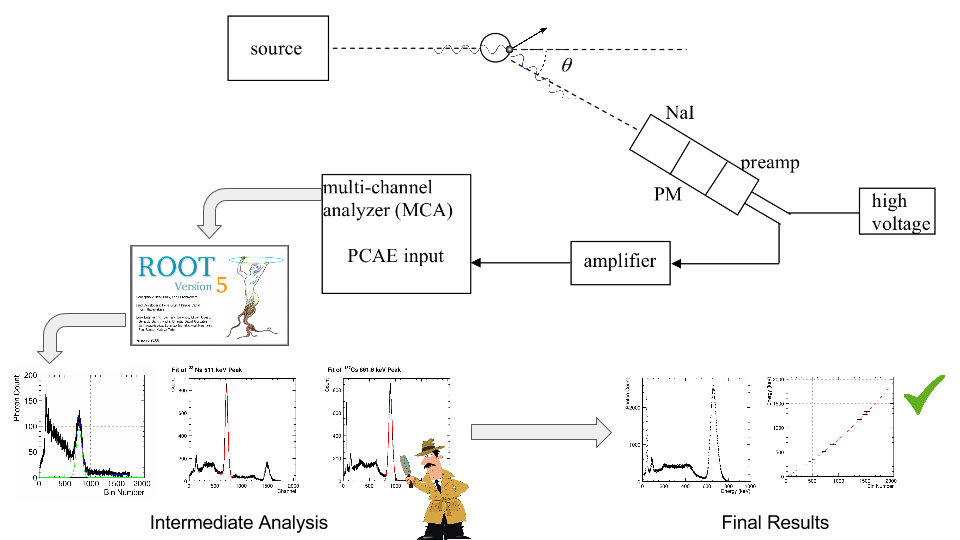
\includegraphics[width=0.5\textwidth]{Setup_full.png}
	\caption{Experimental Setup, modified from Figure 1 in \cite{manual}.}
	\label{Setup}
\end{figure}

\section{Measurements}

\subsection{Calibration of Detector Energy Scale}
Before the gamma ray scattering from $^{137}Cs$ can be analyzed an energy calibration of the MCA program is required. This is done through analysis of the histograms generated by the data provided by the program. As previously mentioned, the MCA program stores a count of the events in each channel which can be plotted as a histogram. The peaks on such a histogram indicate the more frequent energies of photons emitted by the source. These peaks can be fit to a Gaussian function (sometimes with a background function) to find the mean value of the peak and a standard deviation. For many different sources, the mean value of these peaks can be identified as an energy value known to be characteristic of the spectrum of the source. As an example, the peak of the $^{137}Cs$ spectrum fitted in Fig.\ref{Fig:CsUncalib} is associated with an energy value of 661.6 keV. Fig.\ref{Fig:Na511Fit} demonstrates another example, with a fit of the 511 keV peak associated with electron-positron annihilation.

\begin{figure}[H]
\centering	
	\centering	
	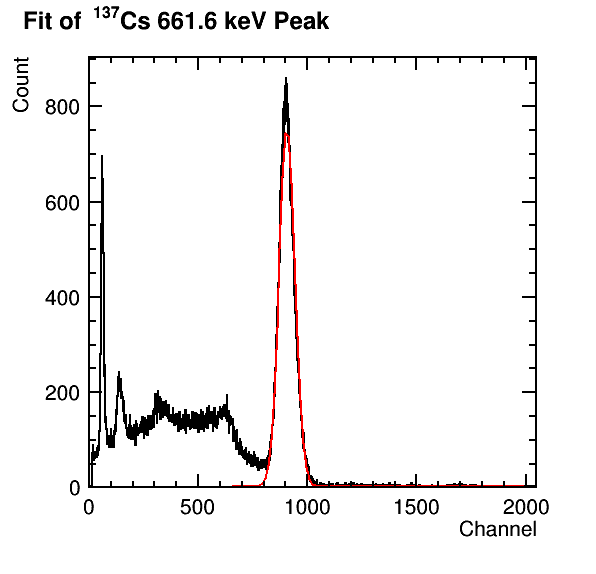
\includegraphics[width=0.4\textwidth]{Cs662keVFit.png}
	\caption{Fit of 661.6 keV Peak on $^{137}Cs$ Spectrum using Gaussian Function and a Background Exponential Decay}
	\label{Fig:CsUncalib}
\end{figure}

\begin{figure}[H]
\centering	
	\centering	
	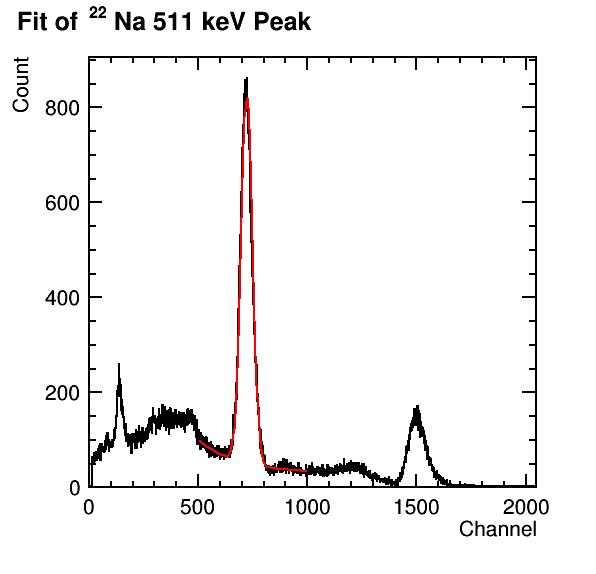
\includegraphics[width=0.4\textwidth]{Na511keVFit.png}
	\caption{Fit of 511 keV Peak on $^{22}Na$ Spectrum using Gaussian Function and a Background Exponential Decay}
	\label{Fig:Na511Fit}
\end{figure}

An energy calibration can be determined by plotting several energy vs channel points from different sources on a graph and fitting the graph to some function. Fig.\ref{Fig:EvBin} shows the plot generated for this experiment.

\begin{figure}[H]
\centering	
	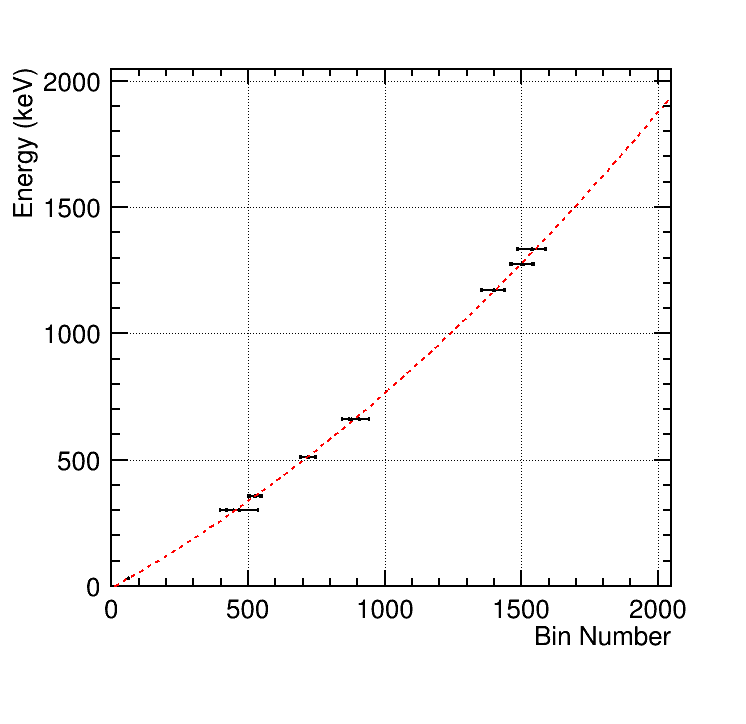
\includegraphics[width=0.4\textwidth]{BinvEnergy.png}
	\caption{Energy vs Bin Calibration Plot}
	\label{Fig:EvBin}
\end{figure}

The fit on the calibration plot in Fig.\ref{Fig:EvBin} is a quadratic fit of the form:
\begin{equation*}
f(x) = [0] + [1]*x + [2]*x^{2}
\end{equation*}
In an ideal setup, the detector and electronics would yield a linear relationship between channel number ($n$) and energy ($E$), but due to small non-linearities in the electronics of this setup, this relationship turns out to be quadratic with an exact formula of:

\begin{equation*}
E = 0.000170654 n^2 + 0.600313 n - 5.13889
\end{equation*}

From this formula, the histograms can be calibrated to yield a correct energy scale such as the $^{137}Cs$ spectrum in Fig.\ref{Fig:CsCalib}. These histograms can then be used for data analysis of the angular dependence of the differential cross section of Compton scattering.
\begin{figure}[H]
\centering	
	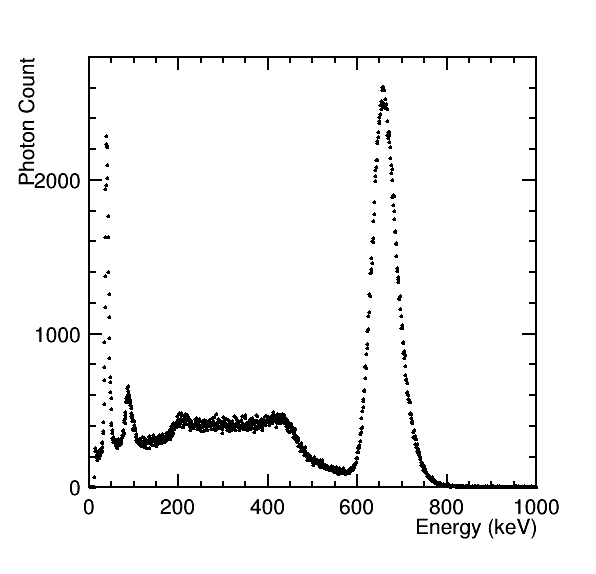
\includegraphics[width=0.4\textwidth]{CsCalibFullSpec.png}
	\caption{}
	\label{Fig:CsCalib}
\end{figure}

\subsection{Electron Rest Mass}

Once the calibrated energy scale of the collected data is determined, the angular dependence of the kinematics of Compton Scattering can be verified by placing the detector at various angles from the beam axis of the gamma ray source. The first value to verify is the energy of the scattered photon. As previously mentioned, this energy follows the relationship defined in Eq. \ref{eq:energy_scatter}. Taking the inverse of each side orients the equation into a form that allows for more straight forward data analysis.

\begin{gather*}\label{eq:energy_scatter2}
	\frac{1}{E_\gamma '} = \frac{1}{E_\gamma} + \frac{1}{m_{e}c^{2}}(1 - cos\theta)
\end{gather*}

This form of the equation demonstrates a linear relationship between $\frac{1}{E_\gamma '}$ and $(1 - \cos\theta)$ with a slope of $\frac{1}{m_{e}c^{2}}$. Plotting the measured energy of the scattered photon as a function of the angle of the detector yields a plot similar to the one in FIG.~\ref{Fig:EScatFit}.

\begin{figure}[H]
\centering	
	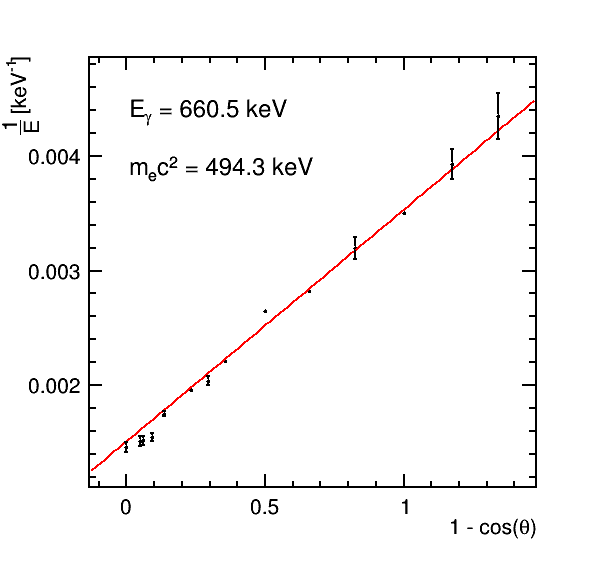
\includegraphics[width=0.4\textwidth]{EScatvTheta.png}
	\caption{Plot of relationship between scattered photon energy ($E_\gamma$) and angle ($\theta$)}
	\label{Fig:EScatFit}
\end{figure}

FIG.~\ref{Fig:EScatFit} shows a linear fit applied to the experimental data (shown in red). Using the intercept of this fit, the initial energy of the gamma photon was calculated to be $E_\gamma = 665.064 \pm 32.243 keV$ which is consistent with the expected value of $661.5keV$. The slope of this fit can be used to calculate the rest mass of the electron $m_{e}c^{2}$. For this experiment, this rest mass was calculated to be $m_{e}c^{2} = 493.859 \pm 36.185 keV$ which is consistent with the expected value of $511 keV$. The data's consistency with the theoretical rest mass of the electron verifies the relationship between scattered photon energy and scattering angle outlined by Eq.~\ref{eq:energy_scatter}.

\subsection{Angular Dependence of the Scattering Probability}

\begin{gather}\label{eq:fitfunction}
	f(x) = [0]*e^{\frac{(x-[1])^2}{2*[2]^2}} + e^{[3]+[4]x} + [5]
\end{gather}

\begin{gather}\label{eq:y_theta}
	Y(\theta) = N_\gamma N_e \frac{d\sigma}{d\Omega}d\Omega \rightarrow \frac{d\sigma}{d\Omega} = \frac{Y(\theta)}{N_\gamma N_e d\Omega}
\end{gather}

After calibrating our detector and using that calibration to determine the electron mass, we sought to understand the angular dependence of the scattering probability for our $\gamma$-rays, or how $d \sigma / d \Omega$ changes with $\theta$. In order to do this, we placed the large Al scatterer at the pivot point of our setup and took spectra of the strong $^{137}$Cs source. We positioned thick blocks of lead to obscure the source from the detector, so that the vast majority of $\gamma$-rays we would detect would be those which had scattered through the aluminum. We measured the resulting spectra, multiple times, at a number of angles between $0^{\circ}$ and $110^{\circ}$. Using Eq. \ref{eq:y_theta}, defined in \cite{milissinos} and \cite{manual}, we can use these spectra to relate the number of photons observed to $d\sigma / d\Omega$. At each angle, we fit the $661.6~keV$ peak to Equation \ref{eq:fitfunction} and integrated over the gaussian portion of our fit (The green curve in Figure \ref{GaussianPortion}), discarding the background photons. We then normalized each spectra for the amount of time the measurement took, as the lower angles would take only a few seconds while the higher angles would take upwards of 30 minutes to get the same number of counts in the peak bins.

\begin{figure}[H]
	\centering
	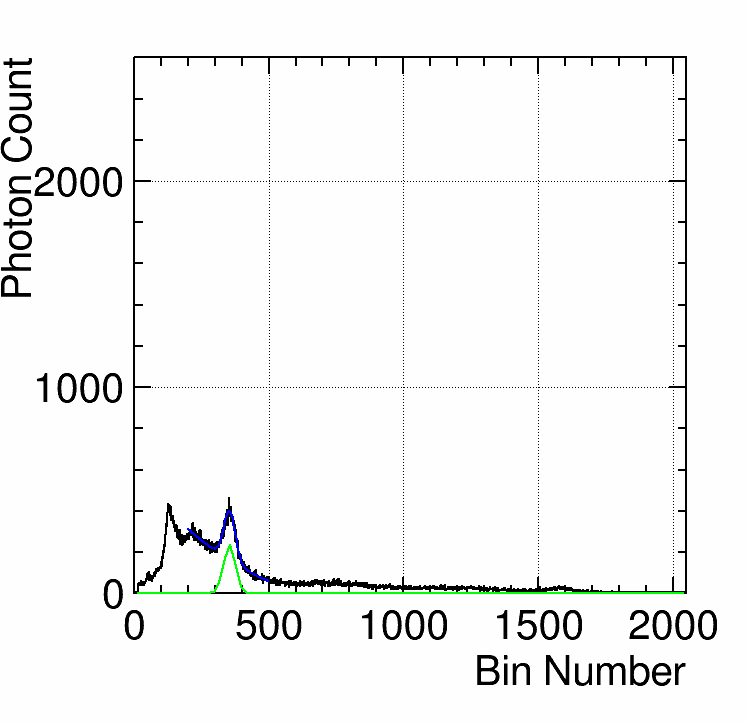
\includegraphics[width=0.4\textwidth]{GaussianPortion.png}
	\caption{Plot showing the total fit (blue) and gaussian fit (green) for the spectrum of $^{137}$Cs at $\theta = 30^\circ$.}
	\label{GaussianPortion}
\end{figure}

This integral gives us our value for $Y(\theta)$. $N_\gamma$ is found in much the same way, but at $\theta = 0^\circ$ and with the scatterer absent. To obtain the value of $d\Omega$, we simply measured the area of the detector and the distance from the source to the detector. From these values, the angle subtended by the detector is simply: $d\Omega = A_{det}/r^2$. We then needed to estimate the number of electrons $N_e$ in the scatterer. For this portion of the experiment, we assume that all of the electrons in the Aluminum are free. With this assumption, the expression for $N_e$ reduces to:
\begin{gather}
	\begin{split}
		N_e 		& = \pi*\left(\frac{d_{scatter}}{2}\right)^2*h_{scatter}*\rho_{Al}*\frac{N_A}{A_{Al}}*Z_{Al} \\
				& = 4.29014*10^{26} \text{ electrons}
	\end{split} \nonumber
\end{gather}
\noindent Having determined all of these values, we created a plot of our experimentally determined $d\sigma / d\Omega$ vs. $\theta$, which can be seen in Figure \ref{KN} below:

\begin{figure}[H]
	\centering
	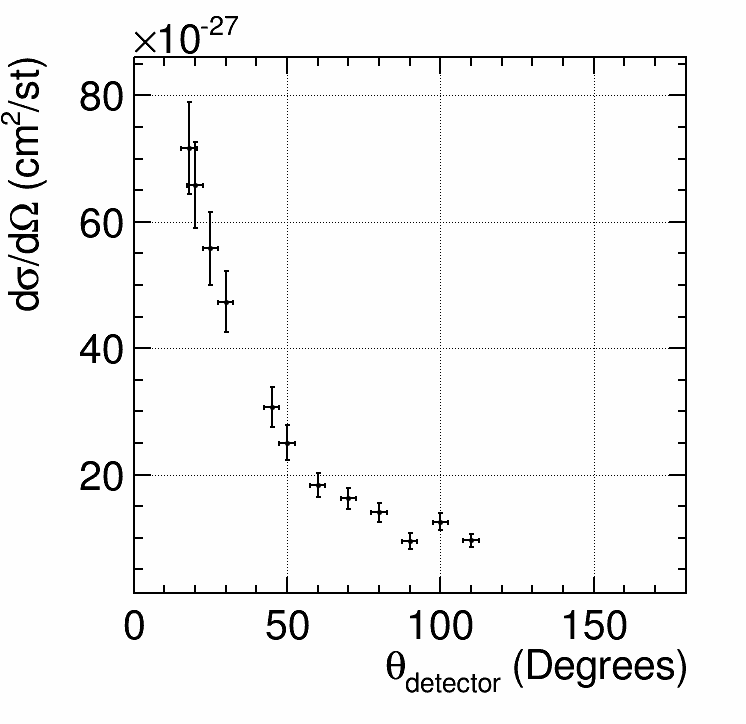
\includegraphics[width=0.4\textwidth]{KNvsThompson_DataOnly.png}
	\caption{Data from experimental measurement of $d\sigma/d\Omega$.}
	\label{KN}
\end{figure}

\noindent At a glance, we can see that the data does not appear to exhibit the $(1 - \cos{\theta})$ dependence predicted by the Thompson formula, a feature most prominent at angles $\ge 90^\circ$, and appears to be roughly consistent with the shape predicted by the Klein-Nishina Formula. The error bars in $d \sigma / d\Omega$ were calculated by propagating through the errors in each of its components (Equation \ref{eq:y_theta}) using techniques from \cite{bevington} and assuming an error in the position of the detector of $\pm 2^\circ$ due to the poor markings on the table. A link to a repository containing the source code for these calculations can be found in Appendix \ref{section:analysis_code}. In the coming sections, we will compare this data in a more rigorous way to the results predicted by both the Thompson and Klein-Nishina Formulae.

\subsection{Free Electrons in Cu and Al}

Knowing the scattering cross section of a metal can provide information about the free electrons in that metal. More specifically, the scattering cross sections of metals can be used to compare the number of free electrons in different metals. For this experiment, Compton scattering was used to compare the number of free electrons in aluminum (Al) and the number of free electrons in copper (Cu). The ratio of free electrons in aluminum to free electrons in copper can be found by calculating the ratio of the scattering cross section of aluminum to the scattering cross section of copper.
\begin{gather}
\frac{e^{-}_{Al}}{e^{-}_{Cu}} = \frac{\frac{d\sigma}{d\Omega}_{Al}}{\frac{d\sigma}{d\Omega}_{Cu}}
\end{gather}
For this experiment, we measured the scattering cross sections of Al and Cu at angles of $25^{\circ}$ and $45^{\circ}$ in order to account for the angular dependence of cross sections. Using the same procedure as in Section 3c, we calculated the scattering cross sections of copper and aluminum at these angles, obtaining the results shown in Table~\ref{Tab:XSecCompare}. 

\begin{table}[htbp]
	\begin{center}
		\begin{tabular}{|c|c|c|c|}
			\hline  & $\frac{d\sigma}{d\Omega}_{1}$ ($10^{-27} m^2$) & $\frac{d\sigma}{d\Omega}_{2}$ ($10^{-27} m^2$) & $\frac{d\sigma}{d\Omega}_{Avg}$ ($10^{-27} m^2$) \\
			\hline \begin{tabular}{@{}c@{}}Al \\ $25^{\circ}$ \end{tabular} & $1.083 \pm 0.054$ & $1.159 \pm 0.058$ & $1.121 \pm 0.079$\\
			\hline \begin{tabular}{@{}c@{}}Cu \\ $25^{\circ}$ \end{tabular}  & $0.4131 \pm 0.0207$ & $0.4322 \pm 0.0216$ & $0.4228 \pm 0.0299$\\
			\hline \begin{tabular}{@{}c@{}}Al \\ $45^{\circ}$ \end{tabular}  & $0.6836 \pm 0.0342$ & $0.6255 \pm 0.0313$ & $0.6546 \pm 0.0464$\\
			\hline \begin{tabular}{@{}c@{}}Cu \\ $45^{\circ}$ \end{tabular}  & $0.2703 \pm 0.0135$ & $0.2094 \pm 0.0105$ & $0.2399 \pm 0.0171$\\
			\hline
			
		\end{tabular}
	\end{center}
	\caption{Scattering Cross Sections of Aluminum and Copper at Varying Angles}
	\label{Tab:XSecCompare}
\end{table}

Using these to calculate the Al-Cu ratio of free electrons yields $ \frac{e^{-}_{Al}}{e^{-}_{Cu}} = 2.65 \pm 0.26$ for $25^{\circ}$ and $\frac{e^{-}_{Al}}{e^{-}_{Cu}} = 2.73 \pm 0.27$ for $45^{\circ}$. These two values are consistent with each other, and, as we will discuss later, are consistent with the expected range of values based on theory.

\section{Theoretical Model}

\subsection{Angular Dependence of the Scattering Probability}

\begin{figure}[H]
	\centering
	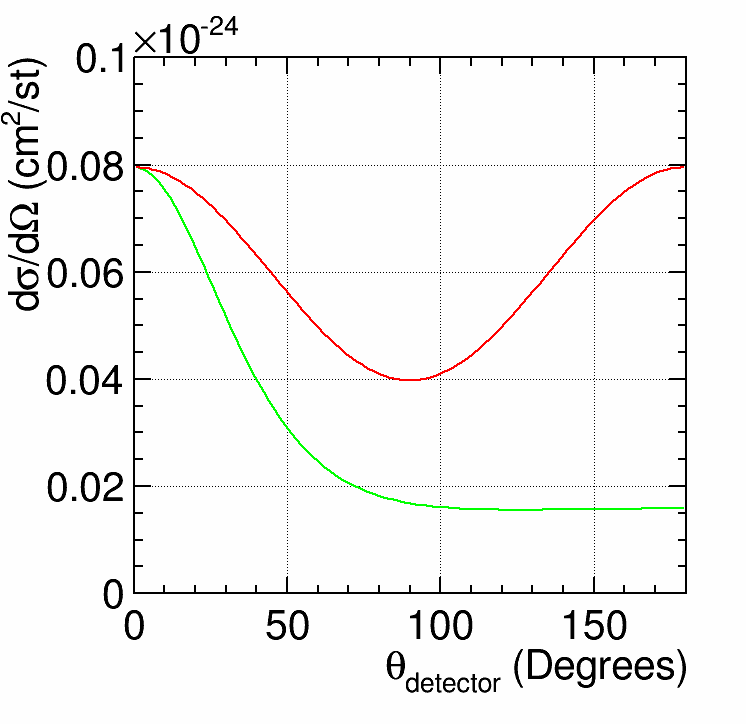
\includegraphics[width=0.4\textwidth]{KNvsThompson_TheoryOnly.png}
	\caption{Comparison of the Theoretical Predictions for the KN and Thompson Models}
	\label{KN_vs_Thompson_Theory}
\end{figure}

Theoretically, the angular dependence of the scattering probability is given by either the Thompson Formula (Equation \ref{eq:thompson}) or the Klein-Nishina Formula (Equation \ref{eq:kn}). While the look completely dissimilar, we can see that the KN formula will converge to the Thompson in the limit of a very low momentum photon. The theoretical predictions for $d\sigma / d\Omega$ for our particular setup is shown in Figure \ref{KN_vs_Thompson_Theory}. This plot shows that at low $\theta$, for a $661.6~keV$ $\gamma$-ray from $^{137}$Cs decay, the two Formulae converge. However, since our photon does not satisfy the classical approximation of $\gamma_{KN} \ll 1$, they quickly diverge as one goes to higher and higher angles. Thus it is these higher angles which are the most important for our comparison of theory and experiment, which can be found in the coming section.

\subsection{Free Electrons in Cu and Al}
Compton scattering is an effect of photons interacting with free electrons in a substance so the number of free electrons is directly related to the scattering cross section of the substance. For a metal, such as Cu or Al, the number of free electrons depends on the number of valence electrons of that metal rather than the total number of electrons of the atom. Copper has 29 total electrons, but only has one or two valence electrons. Meanwhile aluminum has 13 total electrons with three of them being valence electrons. This means the ratio of total electrons for aluminum to copper is 0.5 but the ratio of free electrons for aluminum to copper is between 1.5 and 3.0 depending on the type of copper ions ($Cu^{+1}$ or $Cu^{+2}$) in the metal. As is discussed later, comparison of the scattering cross sections of copper and aluminum shows that the number of valence electrons determines the cross section of a metal, not the total number of electrons.

\section{Comparison of Theory and Experiment}

\subsection{Angular Dependence of the Scattering Probability}

In Figure \ref{KN_vs_Thompson_Unscaled}, we have plotted the data taken during our measurements on top of the Klein-Nishina and Thompson curves:

\begin{figure}[H]
	\centering
	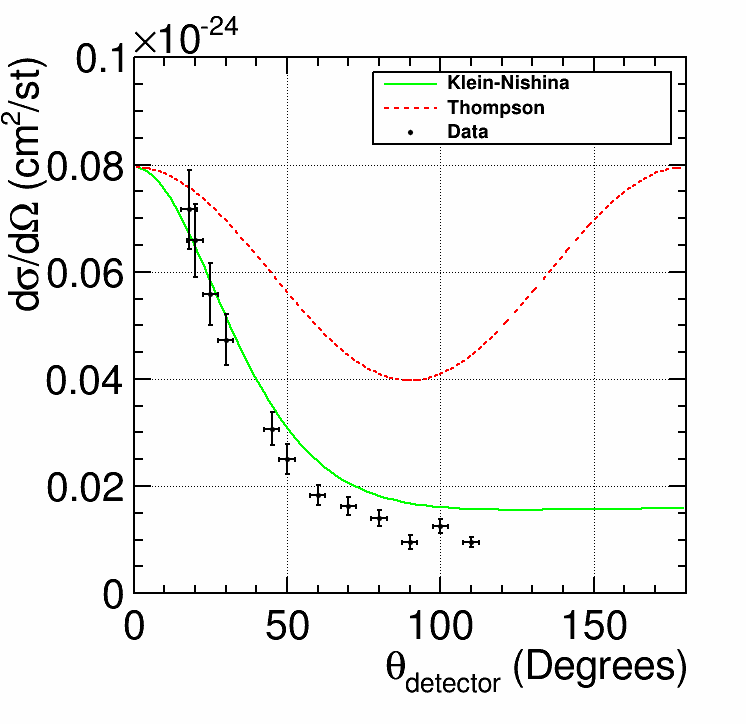
\includegraphics[width=0.4\textwidth]{KNvsThompson_Unscaled.png}
	\caption{Comparison of the Theoretical Predictions with Experimental Data}
	\label{KN_vs_Thompson_Unscaled}
\end{figure}

\noindent From this plot, we can clearly see that the Klein-Nishina Formula is much more consistent with our experimental results then the Thompson Formula, crucially at higher angles. This is in line with our predictions that the more advanced quantum mechanical model would win out over the classical model. In order to quantify how well these functions correspond our data, we used their functional forms as a fit to our data. We found the $\chi^2$ for the two formulae under two conditions, without any additional free parameters and with the addition of an overall scaling term. The results of the $\chi^2$ minimization can be seen in Table \ref{table:chi_square} below:

\begin{table}[htbp]
	\begin{center}
		\begin{tabular}{|l|r|r|}
			\hline
			Function & \multicolumn{1}{l|}{$\chi^2$ (No Parameters)} & \multicolumn{1}{l|}{$\chi^2$ (w/ Parameters)} \\ \hline
			\textit{Thompson} & 193.964 & 2.83089 \\ \hline
			\textit{KN} & 8.54703 & 0.657192 \\ \hline
		\end{tabular}
	\end{center}
	\caption{Comparison of the reduced $\chi^2$ value for the two functions, with and without free parameters.}
	\label{table:chi_square}
\end{table}

\noindent Clearly, Klein-Nishina is more consistent with the data both before and after the addition of a free parameter. However, neither fit has a perfectly reduced $\chi^2$, for a variety of factors. Throughout our analysis, it became apparent that our low angle values of $d\sigma / d\Omega$ were too high and the high angle values were too low, compared to our expectations. This discrepancy changed the shape of our graph from the ideal KN form and made it so that the $\chi^2$ could not be reduced to $\sim 1$. A likely cause of this is a discrepancy in our evaluation of $\epsilon$ and $R_{peak-to-total}$, as we had to extract these values from graphs manually. However, once we added in a degree of freedom to account for this small correction, our $\chi^2$ reduced quite well, and our measurements became superbly consistent with the theoretical predictions of KN.

\subsection{Electron Rest Mass}
In this experiment, we measured the relationship between the scattered photon energy $E_{\gamma}$ and the scattering angle $\theta$ to test Eq.~\ref{eq:energy_scatter}.
\begin{gather*}
	E_\gamma ' = \frac{E_\gamma}{1 + \frac{E_\gamma}{m_e c^2} (1 - \cos{\theta})}
\end{gather*}
When the inverse is taken of each side of this equation, we can see that there should be a linear relationship between $\frac{1}{E_{\gamma}}$ and $1 - cos(\theta)$. Using the slope of this relationship, we could calculate the rest mass of the electron, for which we obtained a value of $493.859 \pm 36.185 keV$. To verify that our linear fit was consistent with our data, we performed a calculation of the minimum chi-squared and obtained a value of $\chi^{2} = 0.675$.  This measurement of the electron's rest mass is consistent with the theoretical value of $511 keV$. 

\subsection{Free Electrons in Cu and Al}
In this experiment, we obtained measurements of the scattering cross sections of aluminum and copper in order to compare the number of free electrons in each of these metals. These measurements were taken at two different scattering angles, $25^{\circ}$ and $45^{\circ}$. Using the ratio of the metals' cross sections, we calculated the ratio of free electrons to be $\frac{e^{-}_{Al}}{e^{-}_{Cu}} = 2.65 \pm 0.26$ for $25^{\circ}$ and $\frac{e^{-}_{Al}}{e^{-}_{Cu}} = 2.73 \pm 0.27$ for $45^{\circ}$. These values are consistent with the expected values based on theory. The free electrons in a metal refer to the valence electrons of an atom of that metal. Aluminum has three valence electrons and copper typically has one valence electron although it can also have two valence electrons. This means that the ratio of free electrons for aluminum to copper should be somewhere between 3.0 and 1.5, depending on which ion of copper is predominant in the metal. The consistency of these results with the expected values verifies that the scattering cross sections of metals depends on the number of free electrons available. It also confirms that the free electrons in a metal refer to the valence electrons in an atom, not the total number of electrons.

\section{Discussion and Conclusions}

Our first step in this experiment was to calibrate the energy scale used by the MCA program in our setup. This program stored information regarding the energy of detected photons in channels that did not explicitly provide the energy of the photons. In order to figure out the relationship between these channels and photon energy, we measured nuclear decay spectra of several radioactive samples with known energy peaks in the spectra. Using data of energy vs channel number, we could find a relationship between these two values in order to calibrate the spectra we measured for our samples. With this method we identified a quadratic behavior between the energy and channel number. This quadratic relationship was most likely a result of imperfections in the electronics that cause the detection system to be non-linear.

After calibrating the energy scale of our detecting equipment, we measured the scattered photon energy as a function of the scattering angle to identify the relationship between these values. We compared our data to Eq.~\ref{eq:energy_scatter} to confirm that the relationship we observed was consistent with theory. To test this consistency, we calculated the rest mass of the electron $m_{e}c^{2}$ and obtained a value consistent with the theoretical value of $511 keV$ when we considered uncertainties in our measurement. This measurement verifies the dependence of the energy of the scattered photon on the scattering angle expressed in Eq.~\ref{eq:energy_scatter}.

From there, we took our measurements of $Y(\theta)$ vs. $\theta$ and created a plot of $d\sigma / d\Omega$ vs. $\theta$. We found that our data was highly consistent with the quantum mechanical Klein-Nishina equation ($\chi^2 = 0.657$), especially at higher angles where the KN formula diverges from the Thompson formula. This is exactly in line with our hypothesis and is yet another proof of the fact that interactions on the atomic scale are primarily quantum mechanical phenomena, and cannot be treated via classical approximations without gross oversimplification.

This experiment could be improved with a stronger and/or more collimated source. We found that our fitting algorithms struggled to identify a gaussian peak if there were too few counts in the peak bin. Qualitatively, we found the ideal number of counts in the peak to be on the order of 100. For the low angles, this was no problem, and the measurement could be completed in just minutes, but for the higher angles we found ourselves needing over 45 minutes to reach the same count number. Were we to have had a stronger source, our count rate would have been much higher, and our measurement time would have been significantly reduced. This extra time could have been used for extra trials or improving our statistical uncertainties in other ways. This experiment could also have been aided by better markings on the tabletop (or a better system for creating our own). This was a large contributer to our uncertainty in the plots of $d\sigma / d\Omega$ and could have been greatly reduced if we had a trusted angular measurement system similar to the $\gamma$-$\gamma$ correlation experiment.

\section{Author Contributions}

Both authors believe that the work for this project was split equally, and each offered valuable insight to every section of this report. However, the sections when divided up by principle author are as follows:

\noindent \textbf{Joshua LaBounty}:
\begin{enumerate}
	\item Section 1: Background 
	\item Section 2: Experimental Setup
	\item Section 3b, 4a, \& 5a: Angular Dependence of the Scattering Probability
	\item Appendix A: Derivation of Equation \ref{eq:energy_scatter}
\end{enumerate}

\noindent \textbf{Thomas Krahulik}:
\begin{enumerate}
	\item Section 3a: Calibration of Detector Energy Scale
	\item Section 3b \& 5b: Electron Rest Mass
	\item Section 3d: Free Electrons in Cu and Al
	\item Appendix B: Validation of the $\chi^2$ Minimization in ROOT
\end{enumerate}

\noindent Lab time was also split equally, with one partner often taking measurements while the other developed the analysis software used in this report.

\begin{thebibliography}{6}
	
	\bibitem{milissinos}
	A.C. Melissinos, Experiments in Modern Physics (Academic Press, NY, 1966).
	
	\bibitem{bevington}
	Philip R. Bevington and D. Keith Robinson, Data Reduction and Error Analysis 3rd edition (McGraw-Hill, 2003).

	\bibitem{bartlett}
	A. A. Bartlett, Am. J. Phys. 32 , 120 (1964).
	
	\bibitem{compton_paper_original}
	A. H. Compton, Phys. Rev. 21 , 483 and 715 (1923).
	
	\bibitem{manual}
	R. Lefferts, Compton Scattering (2010).
	
	\bibitem{emass_1}
	 S. Prassanakumar, S. Krishnaveni, and T.K. Umesh. Determination of rest mass energy of the electron by a compton scattering experiment. Eur. J. Physics, 33:65–72, 2012.
	 
	\bibitem{emass_2}
	S.B. Hosur and N.M. Badiger. Determination of rest mass energy of an electron - an undergraduate laboratory experiment. Eur. J. Physics, 28:1233–1239, 2007.
	
	\bibitem{emass_3}
	Mudhole T S and Umakantha N 1977 Determination of the rest mass energy of the electron: a laboratory experiment Am. J. Phys. 45 1119
	
	\bibitem{kn_paper_original}
	Klein, O. \& Nishina, Y. Z. Physik (1929) 52: 853. doi:10.1007/BF01366453
	
	\bibitem{angle_1}
	Kim, Tony Hyun. Compton Scattering (2008). MIT Department of Physics.
	
	\bibitem{angle_2}
	Lacoste-Julien, Simon and Plamondon, Mathieu. Compton Scattering: Light reveals its particle nature (2002). McGill University.
	
	\bibitem{angle_3}
	Nelson, Dylan R. and  Cheung, Joey. Compton Scattering (2007). University of California,  Berkeley.
	
	\bibitem{eisberg}
	R. M. Eisberg et al., Chapter 14: X-Rays. Fundamentals of Modern Physics,  (Wiley, 1961), Physics Library Ref. QC173.E38.
	
	\bibitem{nstars}
	J. Madej, A. Różańska, A. Majczyna, M. Należyty. Computations of Compton scattering redistribution function in plasma. arXiv:1602.05088
	
	\bibitem{comptonresearch}
	E B Karlsson, O Hartmann, C A Chatzidimitriou-Dreismann, and T Abdul-Redah. The hydrogen anomaly in neutron Compton scattering: new experiments and a quantitative theoretical explanation (2016). IOP Measurement Science and Technology, Volume 27, Number 8.


\end{thebibliography}

\begin{appendix}

\section{Derivation of Equation \ref{eq:energy_scatter}} \label{section:derivation}

\begin{figure}[H]
	\centering
	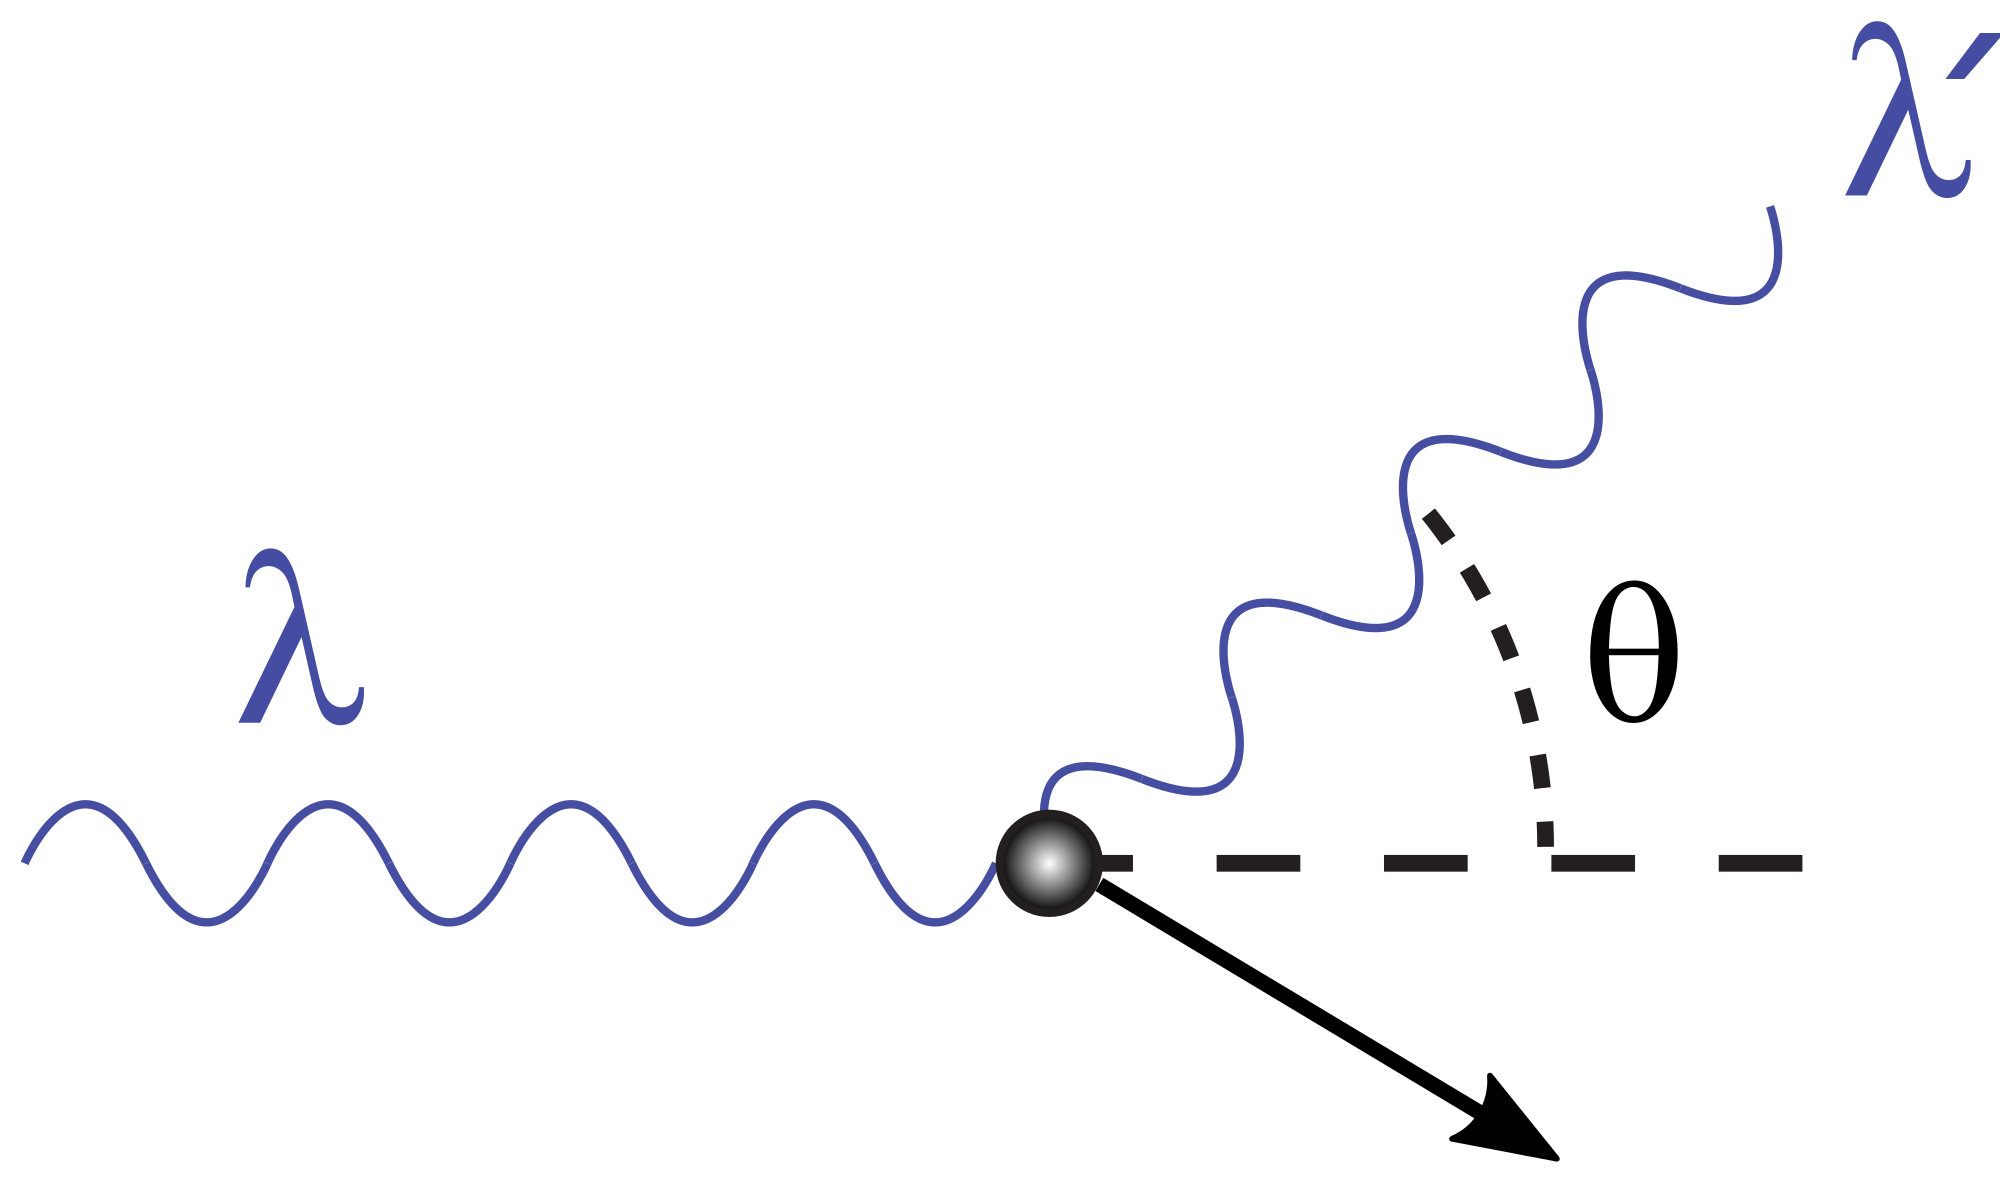
\includegraphics[width=0.3\textwidth]{../plots/ComptonDiagram.png}
	\caption{Diagram showing a photon scattering off an electron at rest. Image courtesy of Wikipedia.}
\end{figure}

This formula can be described semi-classically using only conservation of energy and conservation of momentum. We approximate this interaction as a photon impacting an electron which is currently at rest. We ignore the binding energy of the electron. The conservation laws require that:

\begin{gather}
	E_\gamma + E_e = E_\gamma ' + E_e '\nonumber \\
	\mathbf{p}_\gamma = \mathbf{p}_\gamma' + \mathbf{p}_e' \nonumber
\end{gather}
Initially:
\begin{gather}
	E_e = m_e c^2 \nonumber
\end{gather}
And after the collision:
\begin{gather}
	E_e' = \sqrt{(\mathbf{p}_e' c)^2 + (m_e c^2)^2} \nonumber
\end{gather}
Substituting these quantities into conservation of energy, we find:
\begin{gather}
	E_\gamma + m_e c^2 = E_\gamma' + \sqrt{(\mathbf{p}_e' c)^2 + (m_e c^2)^2} \nonumber \\
	\downarrow \nonumber \\
	\mathbf{p}_e^{2'} c^2  = (E_\gamma - E_\gamma' + m_e c^2)^2 - m_e^2 c^4 \nonumber
\end{gather}
Now returning to conservation of momentum:
\begin{gather}
	\mathbf{p}_e' = \mathbf{p}_\gamma - \mathbf{p}_\gamma' \nonumber
\end{gather}
Since these momenta are vector quantities, and we are only interested in a scalar, we can take the dot product:
\begin{gather}
	p_e^{2'} = \mathbf{p}_e' \cdot \mathbf{p}_e' = p_\gamma^2 + p_\gamma^{2'} - 2 p_\gamma p_\gamma' \cos{\theta} \nonumber \\
	p_e^{2'} c^2 =  p_\gamma^2 c^2 + p_\gamma^{2'} c^2 - 2 c^2 p_\gamma p_\gamma' \cos{\theta} \nonumber \\
	p_e^{2'} c^2 = E_\gamma^2 + E_\gamma^{2'} - 2 E_\gamma E_\gamma' \cos{\theta} \nonumber
\end{gather}
We can now equate these two equations for $p_e^{2'} c^2$ and find:
\begin{gather}
	(E_\gamma - E_\gamma' + m_e c^2)^2 - m_e^2 c^4 = E_\gamma^2 + E_\gamma^{2'} - 2 E_\gamma E_\gamma' \cos{\theta} \nonumber
\end{gather}
We then complete the square and reduce this equation in order to find:
\begin{gather}
	2 m_e c^2 (E_\gamma - E_\gamma') = 2 E_\gamma E_\gamma' (1- \cos{\theta}) \nonumber
\end{gather}
Which we rearrange to arrive back at Equation \ref{eq:energy_scatter}:
\begin{gather}
	E_\gamma ' = \frac{E_\gamma}{1 + \frac{E_\gamma}{m_e c^2} (1 - \cos{\theta})} \nonumber
\end{gather}
Compton's original formulation of this equation is just another form of this equation, rearranging some terms and substituting $\lambda$ for $E_\gamma$ using the relation $E_\gamma = hc/\lambda$.
\begin{gather}
	\lambda' = \lambda + \frac{h}{m_e c} (1 - \cos{\theta}) \nonumber
\end{gather}

\section{Validation of the $\chi^2$ Minimization in ROOT} \label{section:root}

\section{Analysis Code} \label{section:analysis_code}

All of the analysis code used for this lab can be found in the following git repository: 
\begin{verbatim}
https://github.com/jlabounty/SeniorLab/tree
/master/Compton
\end{verbatim}

\end{appendix}

\end{document}


































